\documentclass{beamer}

\usepackage{beamerthemesplit}
\usepackage{graphicx}
\usepackage{subfigure}
\usepackage{amsmath,amssymb}
\usepackage{multimedia}
\usepackage{times}

\usepackage[latin1]{inputenc}
\usepackage[T1]{fontenc}
\usepackage{listings}
\usepackage{courier}
\usepackage{color}
\usepackage{rotating}

\newcommand{\re}{\text{Re}}
\newcommand{\im}{\text{Im}}
\newcommand{\de}{\mbox{d}}
\newcommand{\eref}[1]{(\ref{#1})}
\newcommand{\ii}{\text{i}}
\newcommand{\ee}{\text{e}}
\newcommand{\mathbi}[1]{\textbf{\em #1}}
\newcommand{\rem}[1]{}

% \newcommand{\heading}[1]{\centerline{\Large #1} \vspace{0.5em}}
\newcommand{\heading}[1]{\frametitle{#1}}

\newcommand{\odeint}[0]{Boost.Odeint}
\newcommand{\thrust}[0]{Thrust}
\newcommand{\vexcl}[0]{VexCL}
\newcommand{\boostcompute}[0]{Boost.Compute}
\newcommand{\viennacl}[0]{ViennaCL}
\newcommand{\cmtl}[0]{Cuda-MTL4}



% Layout specification

% \usetheme{AnnArbor}
% \usetheme{Antibes}
% \usetheme{Bergen}
% \usetheme{Berkeley}
% \usetheme{Berlin}
% \usetheme{Boadilla}
% \usetheme{boxes}
% \usetheme{CambridgeUS}
% \usetheme{Copenhagen}
% \usetheme{Darmstadt}
% \usetheme{default}
% \usetheme{Dresden}
% \usetheme{Frankfurt}
% \usetheme{Goettingen}
% \usetheme{Hannover}
% \usetheme{Ilmenau}
% \usetheme{JuanLesPins}
% \usetheme{Luebeck}
% \usetheme{Madrid}
% \usetheme{Malmoe}
% \usetheme{Marburg}
% \usetheme{Montpellier}
% \usetheme{PaloAlto}
% \usetheme{Pittsburgh}
% \usetheme{Rochester}
% \usetheme{Singapore}
% \usetheme{Szeged}
\usetheme{Warsaw}

% \usecolortheme{albatross}
% \usecolortheme{beaver}
% \usecolortheme{beetle}
% \usecolortheme{crane}
% \usecolortheme{default}
% \usecolortheme{dolphin}
% \usecolortheme{dove}
% \usecolortheme{fly}
% \usecolortheme{lily}
% \usecolortheme{orchid}
% \usecolortheme{rose}
% \usecolortheme{seagull}
% \usecolortheme{seahorse}
% \usecolortheme{sidebartab}
% \usecolortheme{structure}
% \usecolortheme{whale}
% \usecolortheme{wolverine}

% \usefonttheme{default}
% \usefonttheme{professionalfonts}
% \usefonttheme{serif}
% \usefonttheme{structurebold}
% \usefonttheme{structureitalicserif}
% \usefonttheme{structuresmallcapsserif}

% \useinnertheme{circles}
% \useinnertheme{default}
% \useinnertheme{inmargin}
% \useinnertheme{rectangles}
% \useinnertheme{rounded}

% \useoutertheme{default}
% \useoutertheme{infolines}
% \useoutertheme{miniframes}
% \useoutertheme{shadow}
% \useoutertheme{sidebar}
% \useoutertheme{smoothbars}
% \useoutertheme{smoothtree}
% \useoutertheme{split}
% \useoutertheme{tree}






% Meta

\title[Iteratorst]{Iterators and Ranges for numerical problems}
% \subtitle[Iterators]{Solving ordinary differential equations in C++}
\author[Karsten Ahnert]{Karsten Ahnert}
\institute[Ambrosys]{Ambrosys GmbH, Potsdam}
\date{December 6, 2014}
%\logo{\pgfimage[width=2cm,height=2cm]{logo}}
\titlegraphic{\includegraphics[width=4cm]{ambrosys}}
\subject{Subject}
\keywords{Keyword1,Keyword2}

\newcommand{\sectionslide}[1]{\frame{\begin{centerline}{\LARGE #1}\end{centerline}}}




\definecolor{dark-gray}{gray}{0.15}
\definecolor{light-gray}{gray}{0.8}
\definecolor{lighter-gray}{gray}{0.9}

\definecolor{dark-green}{rgb}{0,0.4,0}
\definecolor{dark-red}{rgb}{0.2,0,0}

\newcommand{\highlight}[1]{\bf #1}

\lstset{
         basicstyle=\small\ttfamily, % Standardschrift
         %numbers=left,               % Ort der Zeilennummern
         numberstyle=\tiny,          % Stil der Zeilennummern
         %stepnumber=2,               % Abstand zwischen den Zeilennummern
         numbersep=0pt,              % Abstand der Nummern zum Text
         tabsize=2,                  % Groesse von Tabs
         extendedchars=true,         %
         breaklines=true,            % Zeilen werden Umgebrochen
         frame=single,         
         backgroundcolor=\color{lighter-gray},
         tabsize=2,
         keywordstyle=\color{dark-green},
         identifierstyle=,
         commentstyle=\color{dark-gray}\normalfont\rmfamily\itshape,
         stringstyle=\color{dark-red},
         showspaces=false,           % Leerzeichen anzeigen ?
         showtabs=false,             % Tabs anzeigen ?
         xleftmargin=10pt,
         xrightmargin=10pt,
         framexleftmargin=5pt,
         framexrightmargin=5pt,
         framexbottommargin=4pt,
         language=c++,
         showstringspaces=false      % Leerzeichen in Strings anzeigen ?        
 }
\lstloadlanguages{C++}


% What is shown

\beamertemplatenavigationsymbolsempty
\setbeamertemplate{footline}{}
%\setbeamertemplate{footline}{\insertframenumber}
\setbeamertemplate{headline}{}

\setbeamercolor{palette quaternary}{fg=black,bg=white}
\setbeamerfont{frametitle}{size=\Large}
\setbeamercolor{frametitle}{parent=palette quaternary}
\setbeamertemplate{frametitle}
{
  \vspace{1ex}
  \begin{beamercolorbox}[ht=2ex,wd=\paperwidth]{frametitle}
    \centerline{\insertframetitle}
  \end{beamercolorbox}
}

\parindent0pt


\begin{document}





\frame{
  \titlepage


}



\begin{frame}
  \heading{Outline}

  \tableofcontents
\end{frame}



\section{Motivation and introduction}




\begin{frame}[fragile]
\heading{Motivation}

Problem: Find the root of a function \hspace{2ex} $0=f(x)$

\vspace{0.5ex}
Newtons algorithm: \hspace{2ex} $x_{n+1} = x_n - f(x)/f'(x)$
\vspace{2ex}
  \begin{lstlisting}[basicstyle=\scriptsize\ttfamily]
auto newton( auto x , auto f , auto df ) {
    while( std::abs( f(x) ) > 1.0e-12 )
        x = x - f(x) / df( x );
    return x;
}
double x = 1.0;
auto f = []( auto x ) { return exp( -x*x ) - 0.5 ; };
auto df = []( auto x ) { return -2.0*x * exp( -x*x ); };
double root = newton( x , f , df );
  \end{lstlisting}
\vspace{2ex}
Problems with this code?

\pause
\begin{itemize}
 \item Not optimized. \pause -- Not today!
 \item Raw loops. Sean Parent - ``No raw loops''
 
 \vspace{0.5ex}
 Use algorithms and iterators!
\end{itemize}
 
\end{frame}



\begin{frame}[fragile]
 \heading{Motivation}
 
 Use iterator and ranges for three problems:
 
 \begin{itemize}
  \item Numerical Sequences
  \item Dynamical systems
  \item Convergence algorithms
 \end{itemize}
 
 \vspace{2ex}
 
 Range is a proxy for the algorithm!

\end{frame}




\begin{frame}[fragile]
 \heading{Iterators}
 
 \begin{itemize}
  \item Traverse containers
  \item IO 
  \item Expressing algorithms
 \end{itemize}

\end{frame}


\frame{
  \heading{Iterator types -- Concepts}
  
  \centerline{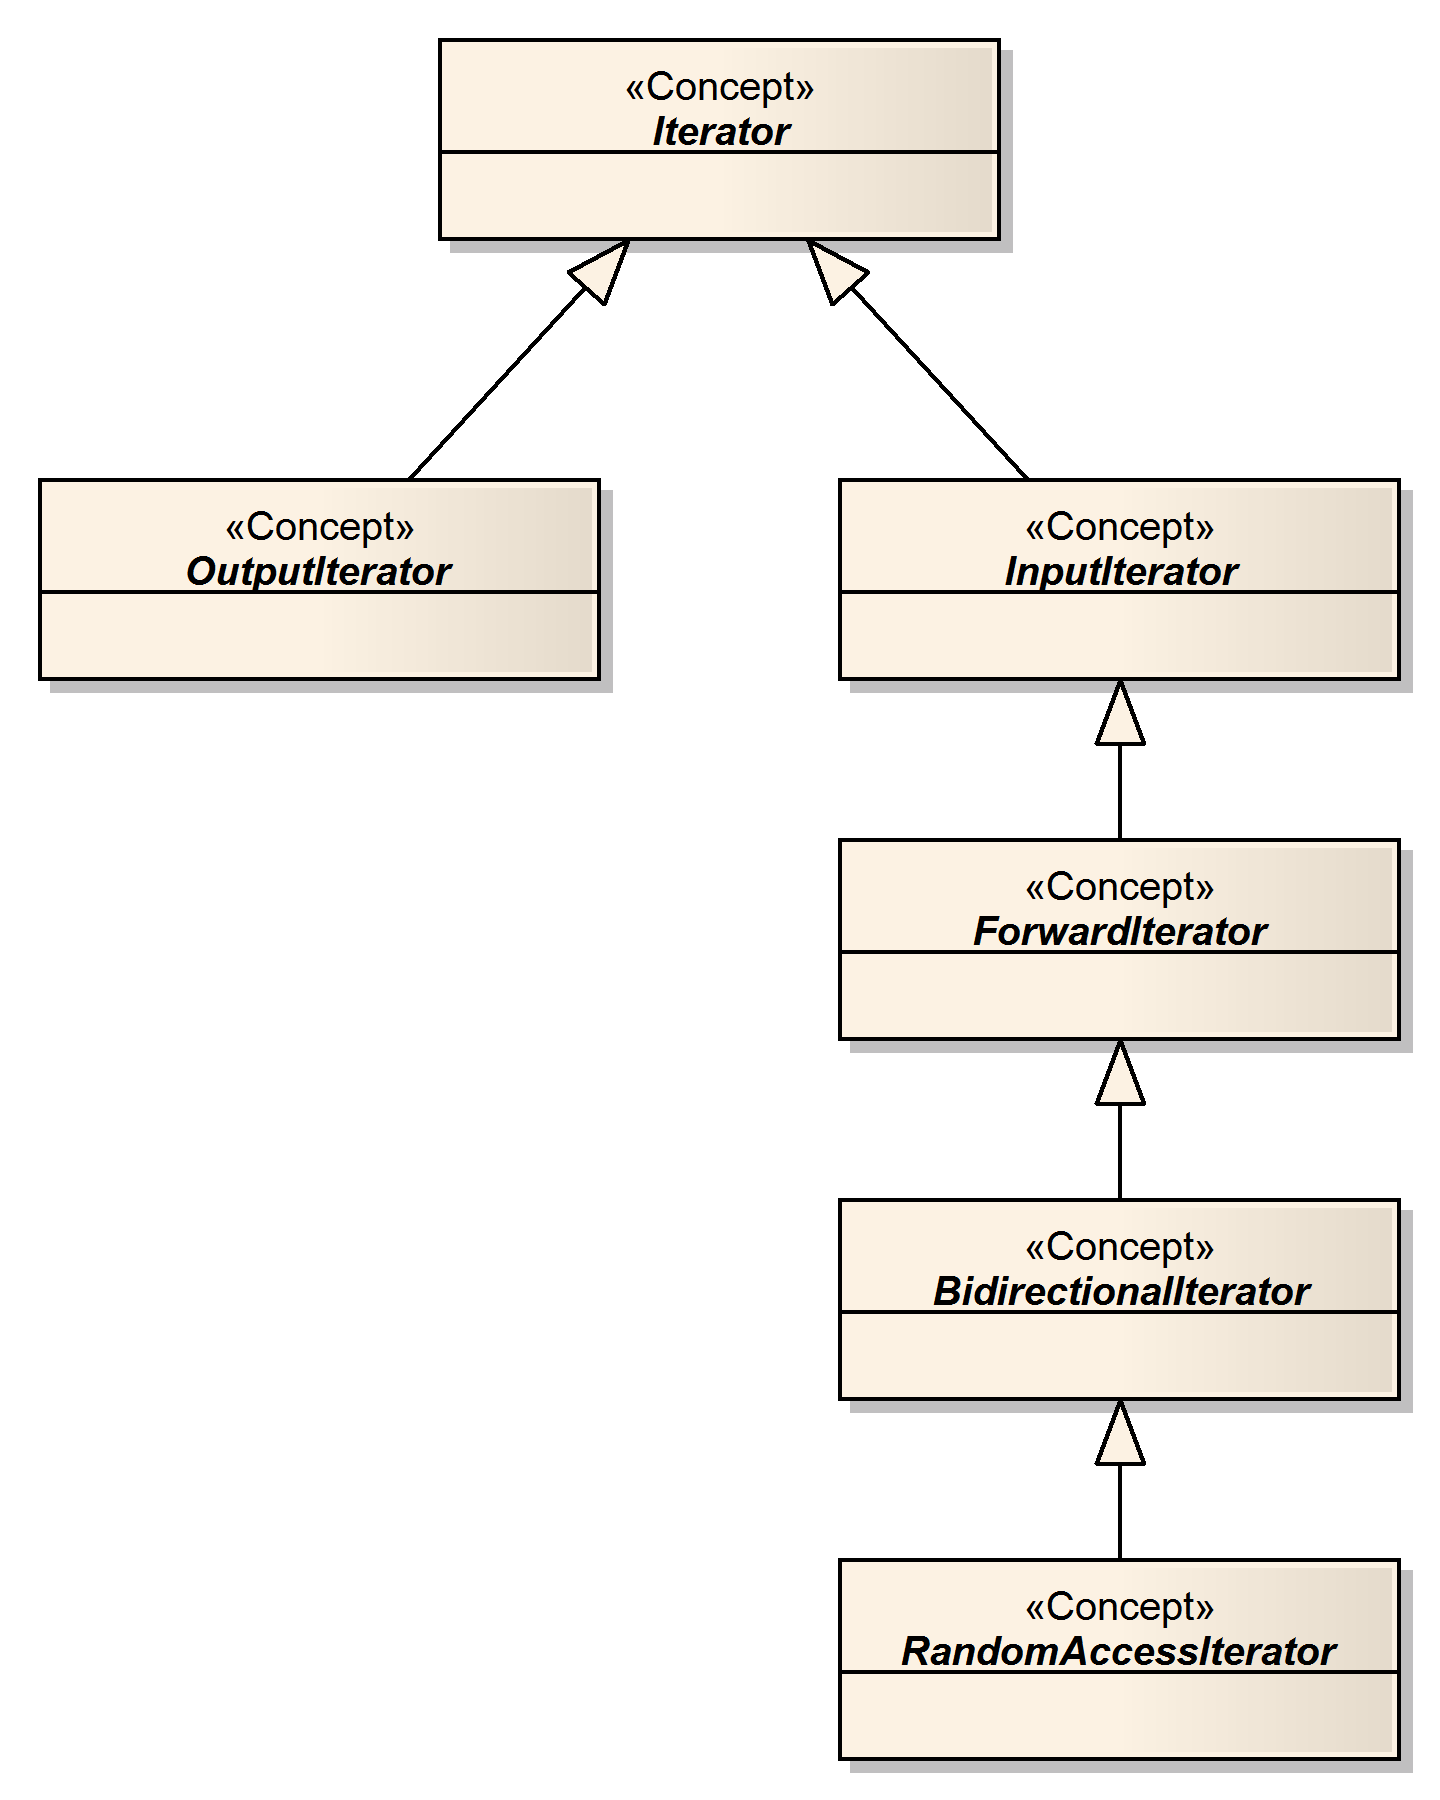
\includegraphics[width=0.5\textwidth]{IteratorsOverview}}
}

\rem{
\begin{frame}[fragile]
  \heading{Iterator types -- Concepts}
  
  \vspace{2ex}
  
  \begin{columns}[T]
    \begin{column}{0.45\textwidth}
      \centerline{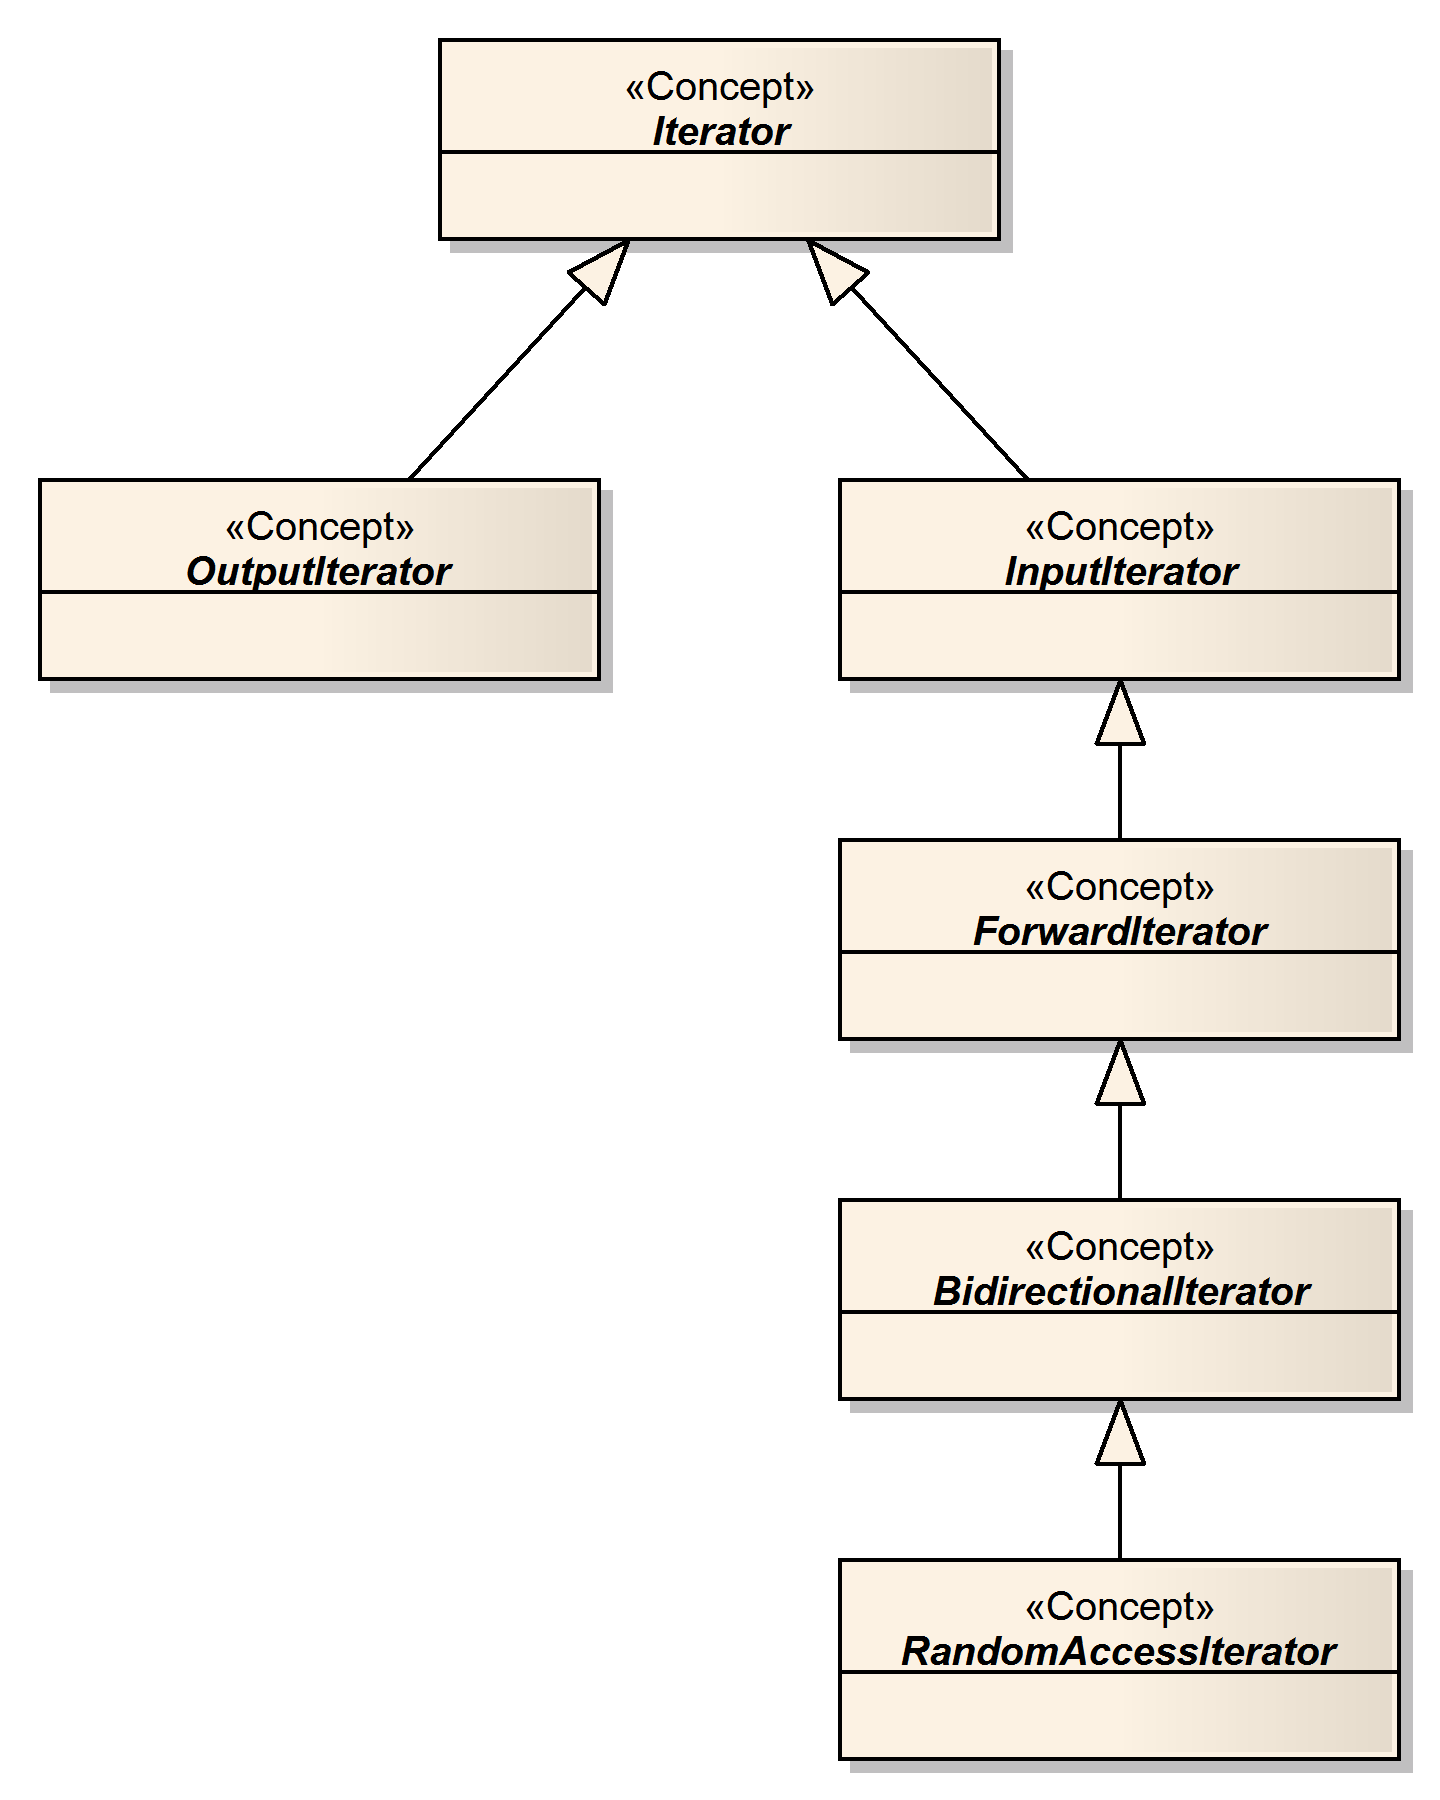
\includegraphics[width=1.0\textwidth]{IteratorsOverview}}
    \end{column}
    \begin{column}{0.55\textwidth}
      \begin{onlyenv}<1>
         OutputIterator
         
         \begin{lstlisting}
*i = o;
*i++ = o;
i++;
++i;
         \end{lstlisting}

         Are special, {\tt back\_inserter}, {\tt ostream\_iterator}, ...
      \end{onlyenv}
      \begin{onlyenv}<2>
         InputIterator a.k.a. Single-Pass Iterator
         
         \begin{lstlisting}
bool r = i != j;
val x = *i;
iterator j = ++i;
i++;
val x = *i++;
         \end{lstlisting}
{\tt istream\_iterator}, {\tt istreambuf\_iterator}

          \vspace{2ex}
          But, if {\tt i == j} then {\tt ++i != ++j}
      \end{onlyenv}
      \begin{onlyenv}<3>
         ForwardIterator
         \begin{lstlisting}
iterator j = i++;
         \end{lstlisting}

          \vspace{2ex}
          But, if {\tt i == j} then {\tt ++i == ++j}
      \end{onlyenv}
      \begin{onlyenv}<4>
         BidirectionalIterator
         \begin{lstlisting}
iterator j = --i;
iterator j = i--;
val x = *i--;
         \end{lstlisting}
         {\tt map< K , V >::iterator, list< T >::iterator}
      \end{onlyenv}
      \begin{onlyenv}<5>
         RandomAccessIterator
         \begin{lstlisting}
i += n;
i -= n;
val x = i[n];
long dist = i - j;
bool b = i < j;
         \end{lstlisting}
         {\tt vector< T >::iterator}
      \end{onlyenv}
    \end{column}
  \end{columns}
\end{frame}
}


\begin{frame}[fragile]
  \heading{Ranges}
  
  \begin{itemize}
   \item Simplifying iterators
   \item Generalization of iterators
   \item Ranges in boost
   \begin{itemize}
    \item Ranges are pairs of iterators.
    \item Ranges can be decorated.
    \item Memory overhead
   \end{itemize}
  \end{itemize}


  \begin{lstlisting}[basicstyle=\scriptsize\ttfamily]
vector< double > values;
// fill values
boost::for_each( values , []( auto x ) {
    cout << x << endl; } );
  \end{lstlisting}


\end{frame}




\frame{
  \heading{Ranges for the C++ standard library}
  
  Eric Niebler: N4128: Ranges for the Standard Library.

  \begin{itemize}
   \item Ranges based on iterators
   \item Introduces new concepts:
   \begin{itemize}
     \item Iterable -- Container, holding the elements 
     \item Range -- Lightweight adapters (decorators)
   \end{itemize}
   \item Several variantes of each algorithm
     \begin{itemize}
       \item sort( in );     
       \item sort( in.begin() , in.end() );
       \item in | view::transform( op );
       \item in | cont::sort( op );       
     \end{itemize}
  \end{itemize}
}


\section{Problem 1 -- Numerical sequences}

\sectionslide{Numerical sequences}

\begin{frame}[fragile]
 \heading{Numerical sequences}
 
 In numerical algorithms one needs often sequences of numerical values
 
 \begin{itemize}
  \item As part of an algorithm
  \item Reference data
  \item Test data
 \end{itemize}

\end{frame}

\begin{frame}[fragile]
 \heading{Numerical sequences}
 
 \begin{onlyenv}<1>
\begin{lstlisting}[basicstyle=\scriptsize\ttfamily]
int n = 1024;
auto seq = boost::counting_range( 0 , n );
for( auto x : seq )
    cout << x << " ";
\end{lstlisting}
\vspace{2ex}Output

\vspace{0.5ex}\lstinline$0 1 2 3 ...$
 \end{onlyenv}
  \begin{onlyenv}<2>
  Range is a proxy object for the sequence
\begin{lstlisting}[basicstyle=\scriptsize\ttfamily]
using namespace boost::adaptors;

auto seq = boost::counting_range( 0 , n );
auto seq2 = seq | transformed( []( auto x ) {
    return 0.1 * static_cast< double >( x ); } );

for( auto x : seq2 )
    cout << x << " ";
\end{lstlisting}
\vspace{2ex}Output

\vspace{0.5ex}\lstinline$0 0.1 0.2 0.3 ...$
 \end{onlyenv}
  \begin{onlyenv}<3>
  Range is a proxy object for the sequence
\begin{lstlisting}[basicstyle=\scriptsize\ttfamily]
auto seq = boost::counting_range( 0 , n );
auto seq2 = seq | transformed( []( auto x ) {
    return 0.01 * static_cast< double >( x ); } );
auto seq3 = seq2 | transformed( []( auto x ) { return sin( 2.0 * x ) + 0.1; } );

for( auto x : seq3 )
    cout << x << " ";
\end{lstlisting}
\vspace{2ex}Output

\vspace{0.5ex}\lstinline$0.1 0.298669 0.489418 0.664642 ...$
 \end{onlyenv}
  \begin{onlyenv}<4>
Use a function
\begin{lstlisting}[basicstyle=\scriptsize\ttfamily]
auto sequence( int n , double sampling , auto f ) {
    auto seq = boost::counting_range( 0 , n );
    return seq | transformed( [sampling,f]( auto x ) { 
        return f(sampling*static_cast<double>( x ) ); } );
}

auto seq = sequence(1024 ,0.1 ,[]( auto x ) {
    return sin(2.0*x)+0.1;} );
for( auto x : seq )
    cout << x << " ";
\end{lstlisting}
\vspace{2ex}Output

\vspace{0.5ex}\lstinline$0.1 0.298669 0.489418 0.664642 ...$
 \end{onlyenv}
 \begin{onlyenv}<5>
  More complicated sequence
\begin{lstlisting}[basicstyle=\scriptsize\ttfamily]
template< typename T >
auto sequence2( int n , double sampling , T f )
{
    auto seq = boost::counting_range( 0 , n );
    return seq | transformed( [sampling,f]( auto i ) {
            double x = sampling*static_cast<double>( i );
            return std::make_tuple(x,f(x)); } );

}

auto seq = sequence2( n , 0.1 , []( auto x ) {
    return sin( 2.0 * x ) + 0.1; } );
for( auto x : zseq )
    cout << "(" << std::get< 0 >( x ) << ","
         << std::get< 1 >( x ) << ") ";
\end{lstlisting}
\vspace{2ex}Output

\vspace{0.5ex}\lstinline$(0,0.1) (0.1,0.298669) (0.2,0.489418) ...$
 \end{onlyenv}
\end{frame}


\begin{frame}[fragile]
  \heading{Numerical ranges and standard C++ Ranges}
  
  Advantages:
  \begin{itemize}
   \item The ranges are natively decorated, not the iterators.
   \item Support for infinite ranges.
  \end{itemize}

 
\end{frame}


\section{Problem 2 -- Dynamical systems}

\sectionslide{Dynamical systems}

\frame{
  \heading{Dynamical systems -- Maps}
  
  \begin{displaymath}
   x_{n+1} = f( x_n )
  \end{displaymath}
  
  \vspace{2ex}
  
  Example: Logistic map
  
  $$ x_{n+1} = r \, x_n ( 1 - x_n ) $$
  
    \centerline{ 
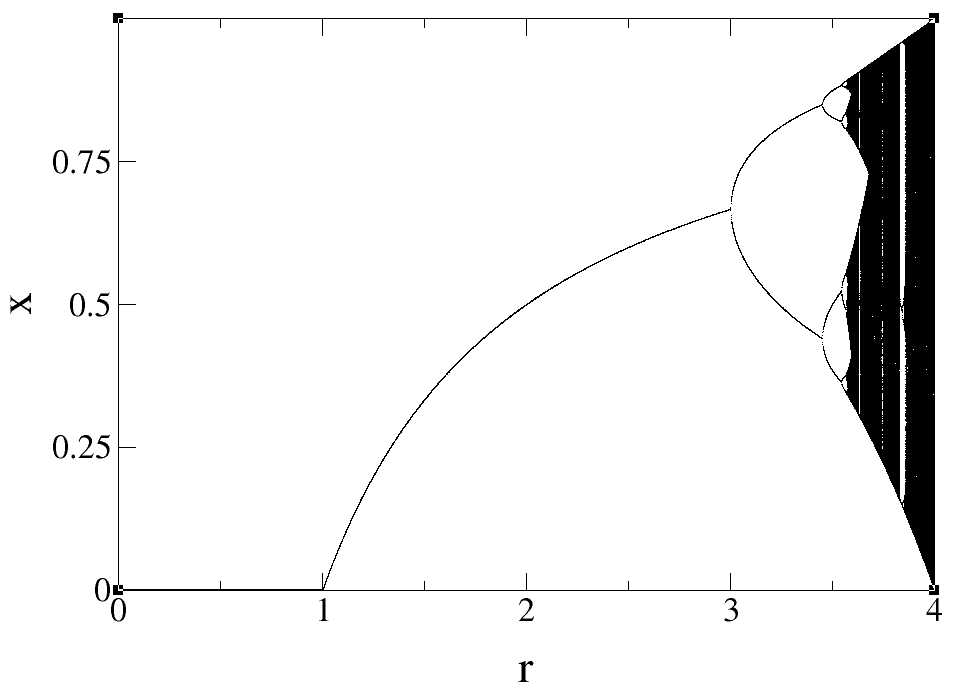
\includegraphics[draft=false,width=0.5\textwidth]{logistic_map}}
}


\frame{
  \heading{Map range}
  
  Abstraction for $x_{n+1} = f(x_n)$
  
  \vspace{2ex}
  
  Two versions:
  
  \begin{enumerate}
   \item {\tt map\_range} - stop predicate 
   \item {\tt counted\_map\_range} - iterates $n$-times
  \end{enumerate}
  
  Models the SinglePassRange concept
}

\begin{frame}[fragile]
  \heading{Map range -- implementation}
  
  \begin{lstlisting}[basicstyle=\scriptsize\ttfamily]
template< typename T1 , ... > class map_range
{
    struct iterator { ... };
 public:
    // ...
    iterator begin() { return iterator( this ); }
    iterator end() { return iterator( nullptr ); }
    // ...
};
   \end{lstlisting}
   
   Range algorithms redirect to iterator algorithms:
   \begin{lstlisting}[basicstyle=\scriptsize\ttfamily]
template< typename R , typename F >
void for_each( R const& r , F f ) {
    std::for_each( r.begin() , e.end() , f );
}
   \end{lstlisting}


\end{frame}



\begin{frame}[fragile]
  \heading{Map range}
  
\begin{lstlisting}[basicstyle=\scriptsize\ttfamily]
template< typename T , typename F , typename C >
class map_range
{
    struct iterator { ... };

  public:
    map_range( T value , F func , C condition )
    : m_value { std::move( value ) }
    , m_func { std::move( func ) }
    , m_condition( condition )
    {}
    
    iterator begin() const { return iterator( this ); }
    iterator end() const { return iterator( nullptr ); }
    
private:
    mutable T m_value;
    mutable F m_func;
    C m_condition;
};
\end{lstlisting}

\end{frame}


\begin{frame}[fragile]
  \heading{Map range}
  
\begin{lstlisting}[basicstyle=\scriptsize\ttfamily]
struct iterator {
    iterator( map_range const* _r ) : r( _r ) {}
    
    iterator& operator++() {
        r->m_value = r->m_func( r->m_value );
        if( r->m_condition( r->m_value ) ) {
            r = nullptr;
        }
        return *this;
    }
    
    T& operator*() const {
        return r->m_value; }
    bool operator==( iterator const& o ) const {
        return ( r == o.r ); }
    bool operator!=( iterator const& o ) const {
        return ! ( *this == o );
    }
    
    map_range const* r;
};
 
\end{lstlisting}

\end{frame}



\begin{frame}[fragile]
  \heading{Counted map range}
  
\begin{lstlisting}[basicstyle=\scriptsize\ttfamily]
template< typename T , typename F >
class counted_map_range
{
    struct iterator { ... };
    
public:
    counted_map_range( T value , F func , size_t max_iterations )
    : m_current_iteration { 0 }
    , m_max_iterations { max_iterations }
    , m_value { std::move( value ) }
    , m_func { std::move( func ) }
    {}
    
    iterator begin() const { return iterator( this ); }
    iterator end( void ) { return iterator( nullptr ); }
    
private:
    mutable size_t m_current_iteration = 0;
    const size_t m_max_iterations;
    mutable T m_value;
    mutable F m_func;
};
\end{lstlisting}

\end{frame}


\begin{frame}[fragile]
 \heading{Factory functions}
 
\begin{lstlisting}[basicstyle=\scriptsize\ttfamily]
template< typename T , typename F , typename C >
auto make_map_range( T t , F f , C condition )
{
    return map_range< T , F , C >(
        std::move( t ) ,
        std::move( f ) ,
        std::move( condition ) );
}
\end{lstlisting}

\begin{lstlisting}[basicstyle=\scriptsize\ttfamily]
template< typename T , typename F >
auto make_counted_map_range( T t , F f , size_t max_iterations )
{
    return counted_map_range< T , F >(
        std::move( t ) ,
        std::move( f ) , 
        max_iterations );
}
\end{lstlisting}

\end{frame}


\begin{frame}[fragile]

  \heading{Example - logistic map}

\begin{lstlisting}[basicstyle=\scriptsize\ttfamily]
double r = 3.2;
auto l = [r]( auto x ) {return r * x * ( 1.0 - x ); };
auto range = make_counted_map_range( 0.5 , l , 1000 );
for( auto x : range ) { cout << x << endl; }
\end{lstlisting}
 
\end{frame}



\begin{frame}[fragile]
 \heading{Dynamical system -- cellular automaton}
 
 Cellular automaton: Time-discrete and value-discrete
 
 \vspace{2ex}
 Conway's Game of Life
 
 \begin{itemize}
  \item Each cell has two states: {\it alive} or {\it dead}
  \item Transition rules
  \begin{itemize}
    \item Less then two neighbors -> dead (under-population)
    \item Two or three neighbors -> alive 
    \item More then three neighbors -> dead (over-population)
    \item Dead cell with three neighbors -> alive (reproduction)
  \end{itemize}
 \end{itemize}
 
 Pictures

\end{frame}

\begin{frame}[fragile]
 \heading{Conway's game of life}
 
 \begin{lstlisting}[basicstyle=\scriptsize\ttfamily]
using board = vector< vector< bool > >;

auto show_board = []( board const& b ) { ... }
auto next_board = []( board const& b ) -> board { ... }

board b;
// initialize b
auto r = make_counted_map_range( b , next_board , 1000 );
for( auto b : r )
{
    show_board( b );
}
 \end{lstlisting}

\end{frame}




\frame{
  \heading{Dynamical systems -- ODEs}
  
  \begin{displaymath}
   \frac{\de x}{\de t} = f( x , t )
  \end{displaymath}
  
  \vspace{2ex}
  
  Example: Lorenz attractor
  
  $$\dot{x} = \sigma(y-x ) \quad \text{,} \quad 
\dot{y} = x ( \rho - z ) - y \quad \text{,} \quad \dot{z} = xy - \beta z$$

 \centerline{ 
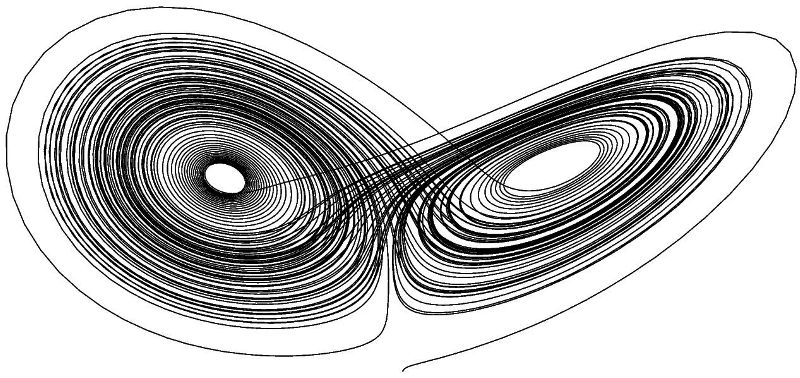
\includegraphics[draft=false,width=0.6\textwidth]{lorenz.jpg}}

  Numerical solution: $x(t+\Delta t) = F( x(t) )$


}


\begin{frame}[fragile]
  \heading{Example -- ODE solver}
  
  Solve $\dot{x} = f(x,t)$, Solver $F$ : $x(t+\delta t)=F(x(t))$
  
  Example \odeint:
  
\begin{lstlisting}[basicstyle=\tiny\ttfamily]
namespace odeint = boost::numeric::odeint;

auto lorenz = []( auto const& x , auto& dxdt , auto t )
{
    dxdt[0] = 10.0 * ( x[1] - x[0] );
    dxdt[1] = 28.0 * x[0] - x[1] - x[0] * x[2];
    dxdt[2] = -8.0 / 3.0 * x[2] + x[0] * x[1];
};

using state_type = std::array< double , 3 >;
odeint::runge_kutta4< state_type > stepper;

state_type x {{ 10.0 , 10.0 , 10.0 }};
double t = 0.0 , dt = 0.01;
stepper.do_step( lorenz , x , t , dt );
t += dt;
  \end{lstlisting}
  
Integrate functions:
\begin{lstlisting}[basicstyle=\tiny\ttfamily]
auto obs = []( auto x , auto t ) { std::cout << t << " " << x[0] << "\n"; };
odeint::integrate_const( stepper , lorenz , x , 0.0 , 10.0 , dt , obs );
\end{lstlisting}

\end{frame}

\begin{frame}[fragile]
 \heading{Example -- ODE solver}
 
 \begin{lstlisting}[basicstyle=\tiny\ttfamily]
auto make_ode_range( auto sys , auto stepper , auto x ,
    auto t0 , auto dt , auto t1 )
{
    auto solve = [sys,stepper,dt]( auto x ) mutable { 
        stepper.do_step( sys , x.first , x.second , dt );
        x.second += dt;
        return x; };
    auto cond = [t1]( auto const& x ) { return x.second > t1; };
    auto range = make_map_range( std::make_pair(x,t0) , solver , cond );
    return range;
}
 \end{lstlisting}
 
 Can be used as
\begin{lstlisting}[basicstyle=\tiny\ttfamily]
state_type x {{ 10.0 , 10.0 , 10.0 }};
stepper_type stepper;
auto range = make_ode_range( lorenz , stepper , x , 0.0 , 0.1 , 100.0 );

for( auto r : range )
    std::cout << r.second << " " << r.first[0] << " " << r.first[1] << "\n"; 
\end{lstlisting}

\end{frame}

\begin{frame}[fragile]
 \heading{ODE ranges}
 
 Superior to integrate functions:
 \begin{itemize}
  \item Break conditions are easy
  \item ODE-Ranges can be used in a natural C++ way, {\tt find}, {\tt 
transform} , etc.
 \end{itemize}
 
 Map implementation has drawbacks -> custom implementation
 \begin{itemize}
  \item Better performance.
  \item Step size control -- complicated iteration.
  \item Break condition can use the last two values.
 \end{itemize}

\end{frame}




\section{Problem 3 -- Convergence methods}

\sectionslide{Convergence methods}




\begin{frame}[fragile]
 
  \heading{Newton method}

  Find the root: $0 = f(x)$
  
  \vspace{2ex}
  
  Newtons method
  
  \begin{itemize}
   \item Choose $x_0$
   \item Iterate $x_{n+1} = x_{n} - \frac{f(x_n)}{f'(x_n)}$
  \end{itemize}

\end{frame}



\begin{frame}[fragile]
 \heading{Newton method -- Implementation}
 
\begin{lstlisting}[basicstyle=\scriptsize\ttfamily]
auto newton_range(
    auto x , auto f , auto df ,
    auto break_condition )
{
    return make_map_range(
        x ,
        [f,df]( auto x ) { return x - f( x ) / df( x ); } ,
        break_condition );
}
\end{lstlisting}

\end{frame}




\begin{frame}[fragile]
 \heading{Newton method -- Example}
 
 Solve $\exp(-x^2) - 0.5 = 0$
 
 \vspace{1ex}
\begin{lstlisting}[basicstyle=\scriptsize\ttfamily]
auto f = []( auto x ) { return exp(-x*x) - 0.5; };
auto df = []( auto x ) { return -2.0*x * exp(-x*x); };
auto cond  = [f]( auto x ) {
    return std::abs(f(x)) < 1.0e-12; };

auto range = newton_range( 1.0 , f , df , cond );

for( auto r : range )
    std::cout << r << " : " << f( r ) << std::endl;
\end{lstlisting}


 \centerline{ 
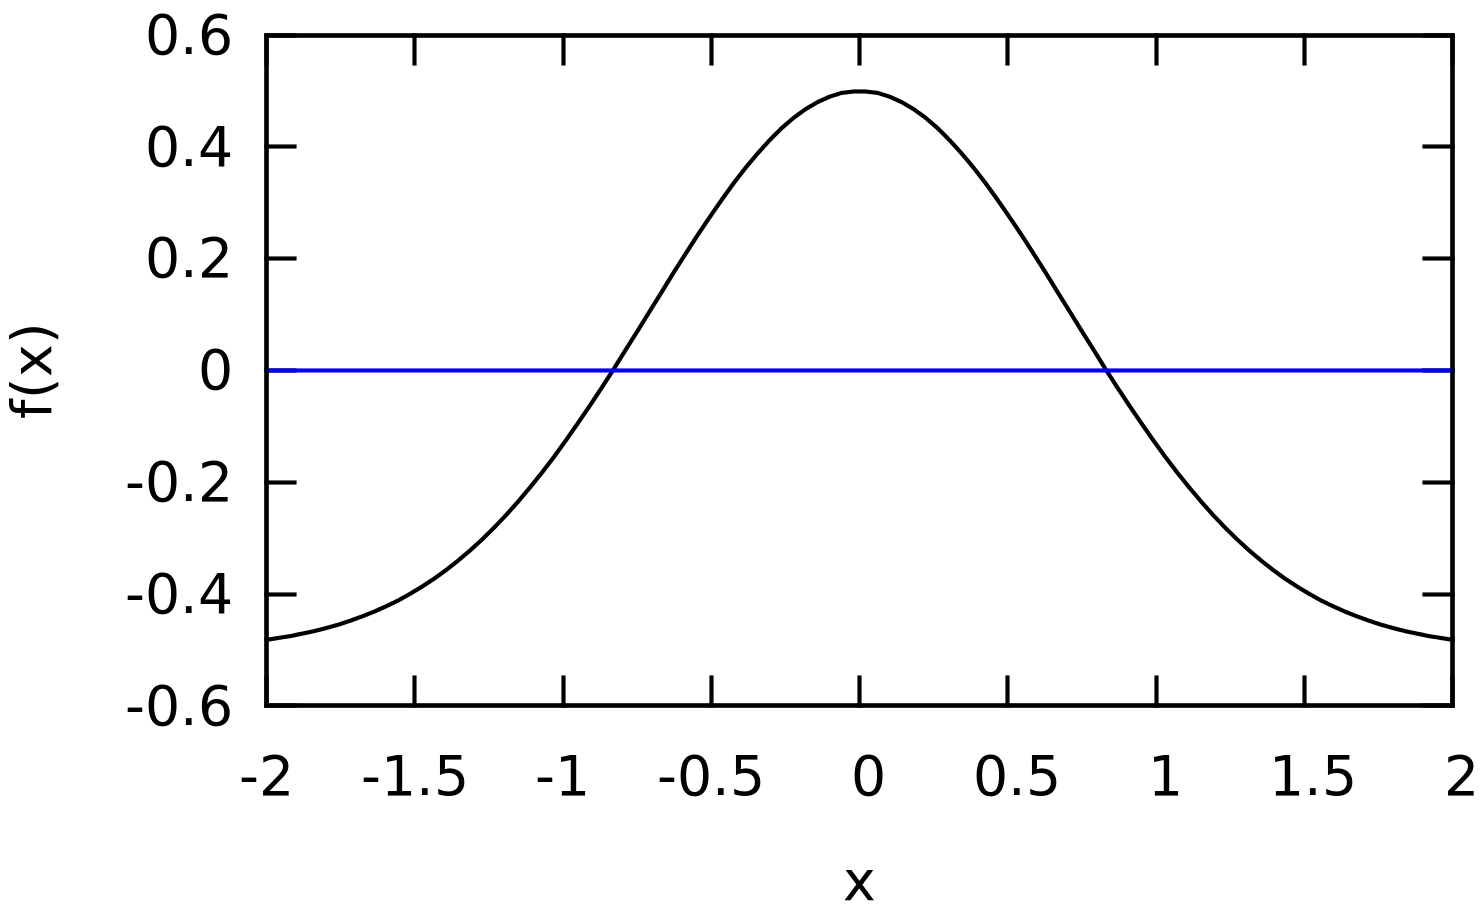
\includegraphics[draft=false,width=0.5\textwidth]{newton1}} 

\end{frame}


\begin{frame}[fragile]
 \heading{Similar problems}
 
 \begin{itemize}
  \item Optimizations methods
  \begin{itemize}
    \item Genetic algorithms, genetic programming, simulated annealing, \dots
  \end{itemize}
  \item Approximation of functions
 \end{itemize}

\end{frame}






\section{Conclusion}

\frame{
  \heading{Conclusion}
  
  \begin{itemize}
   \item Iterators and ranges can be used for numerical problems
   \item For some problems they provide the correct abstraction
   \item If it can be applied to all problems is not clear
   \item The new range library for Standard C++ might ease a lot of things
  \end{itemize}

}



\frame{
  \heading{References}
  
  \begin{itemize}
   \item odeint
   \item github talk
   \item github map range
  \end{itemize}

}







\sectionslide{Backup}


\begin{frame}[fragile]{Example}
 \heading{Example -- basic use}
 \begin{lstlisting}[basicstyle=\scriptsize\ttfamily]
 for( auto iter = values.begin() ;
      iter != values.end() ;
      ++iter )
 {
     cout << *iter << endl;
 }
 \end{lstlisting}
 \pause

 \vspace{2ex}
 C++11 - use range based for
 \begin{lstlisting}[basicstyle=\scriptsize\ttfamily]
  for( auto v : values )
  {
      cout << v << endl;
  }
 \end{lstlisting}

\end{frame}



\begin{frame}[fragile]
 \heading{Example -- Container traversal}
 \begin{onlyenv}<1>
 \begin{lstlisting}
  list< double > values;
  list< double > values2( values.size() );
 \end{lstlisting}
 \end{onlyenv}
 \begin{onlyenv}<2>
 \begin{lstlisting}
  vector< double > values;
  vector< double > values2( values.size() );
 \end{lstlisting}
 \end{onlyenv} 
 \vspace{2ex}
 Can be used in
 \begin{lstlisting}
  transform( values.begin() , values.end() ,
             values2.begin() ,
             []( double x ) {
                 return x * 2.0; } );
 \end{lstlisting}
\end{frame}




\begin{frame}[fragile]
  \heading{Examples -- IO}

Input
\begin{lstlisting}[basicstyle=\scriptsize\ttfamily]
vector< double > values;  
copy_if( istream_iterator< double >( cout ) ,
         istream_iterator< double >() ,
         back_inserter( values ) ,
         []( double x ) { return x > 0.0; } );
\end{lstlisting}
\vspace{2ex}
Output
\begin{lstlisting}[basicstyle=\scriptsize\ttfamily]
vector< double > values;  
// fill values
copy_if( values.begin() , values.end() ,
         ostream_iterator< double >( std::cout , "\n" ) ,
         []( double x ) { return x > 0.0; } );
\end{lstlisting}

\end{frame}








\frame{
  \heading{Algorithms}
  \tiny \tt
  \begin{columns}[T]
   \begin{column}{0.2\textwidth}
      I all\_of \\
      I any\_of \\
      I none\_of \\
      I for\_each \\
      I count \\
      I count\_if \\
      I mismatch \\
      I equal \\
      I find \\
      I find\_if \\
      I find\_if\_not \\
      F find\_end \\
      I,F find\_first\_if \\
      F adjacent\_find \\
      F search \\
      F search\_n \\
      
      I,O copy \\
      I,O copy\_if \\
      I,O copy\_n \\
      B,O copy\_backward \\
      I,O move \\
      B,O move\_backward \\
      F fill \\
      F fill\_n \\
      I,O transform \\
      F generate \\
      I generate\_n \\
   \end{column}
   \begin{column}{0.2\textwidth}
      F remove \\
      F remove\_if \\
      I,O remove\_copy \\
      I,O remove\_copy\_if \\
      F replace \\
      F replace\_if \\
      I,O replace\_copy \\
      I,O replace\_copy\_if \\
      F swap\_ranges \\
      F iter\_swap \\
      B reverse \\
      B,O reverse\_copy \\
      F rotate \\
      F,O rotate\_copy \\
      R random\_shuffle \\
      R shuffle \\
      F unique \\
      I,O unique\_copy
   \end{column}
   \begin{column}{0.3\textwidth}
      I is\_partitioned \\
      F,B partition \\
      I,O partition\_copy \\
      B stable\_partition \\
      F partition\_point \\
      F is\_sorted \\
      F is\_sorted\_until \\
      R sort \\
      R partial\_sort \\
      I,R partial\_sort\_copy \\
      R stable\_sort \\
      R nth\_element \\
      \hrule
      F lower\_bound \\
      F upper\_bound \\
      F binary\_search \\
      F equal\_range \\
      I,O merge \\
      B inplace\_merge \\
      I includes \\
      I,O set\_difference \\
      I,O set\_intersection \\
      I,O set\_symmetric\_difference \\
      I,O set\_unition 
    \end{column}
    \begin{column}{0.3\textwidth}
      \hrule
      R is\_heap \\
      R is\_heap\_until \\
      R make\_heap \\
      R push\_heap \\
      R pop\_heap \\
      R sort\_heap \\
      \hrule
      F max\_element \\
      F min\_element \\
      F minmax\_element \\
      I lexicographical\_compare \\
      F is\_permutation \\
      B next\_permutation \\
      B prev\_permutation \\
      \hrule
      F iota \\
      I accumulate \\
      I inner\_product \\
      I,O adjacent\_difference \\
      I,O partial\_sum
   \end{column}
  \end{columns}


}







\begin{frame}[fragile]
 \heading{Examples -- generalized iota}
 
 Generalized Iota:
\begin{lstlisting}[basicstyle=\scriptsize\ttfamily]
size_t n = 10;
auto iota = make_counted_map_range( 1 , []( auto x ) {
    return x * 2; } , 10 );

std::vector< int > values;
boost::copy( iota_range , std::back_inserter( values ) );
for( auto i : values ) { cout << i << endl; }
\end{lstlisting}

\end{frame}

\begin{frame}[fragile]
  \heading{Examples -- generalized iota}
  
  \textbf{Problem:} We can not easily generate a square iota:
 
  $1,4,9,16,25,36,...$
    
  \pause
 
  Introduce a projected map range.
  
  \begin{lstlisting}[basicstyle=\scriptsize\ttfamily]
auto iota_range = make_projected_counted_map_range(
    1 
    , []( auto x ) { return x+1 ; }
    , 11
    , []( auto x ) { return x*x; }
    );
for( auto i : iota_range ) { std::cout << i << std::endl; }
  \end{lstlisting}


\end{frame}




\frame{
  \heading{Map range - applications}
  
  \begin{itemize}
   \item Generalized iota
   \item Ordinary differential equations
   \item Maps (dynamical maps)
   \item Functional random number generators
   \item Opmization methods
   \begin{itemize}
     \item Genetic algorithms, Simulated annealing, \dots
   \end{itemize}
  \end{itemize}
}




\frame{
  \heading{Map range - applications}
  
  \begin{itemize}
   \item Generalized iota
   \item Ordinary differential equations
   \item Maps (dynamical maps)
   \item Converging algorithms
   \item Functional random number generators
  \end{itemize}
}










\sectionslide{Iterators for GPUs algorithms}

\frame{
  \heading{High-level libraries for GPUs}
  
  \begin{itemize}
    \item Thrust
    \item VexCL
    \item Boost.Compute
    \item ViennaCL
    \item Cuda-MTL
  \end{itemize}
}

\begin{frame}[fragile]
  \heading{Thrust}
  
  Thrust is STL-like library for Cuda -- Based on iterators.
 
  \begin{lstlisting}[basicstyle=\scriptsize\ttfamily]
thrust::host_vector<int> h_vec( 1024 );
std::generate(h_vec.begin(), h_vec.end(), rand);

thrust::device_vector<int> d_vec = h_vec;
thrust::sort(d_vec.begin(), d_vec.end());

thrust::copy(d_vec.begin(), d_vec.end(), h_vec.begin());
  \end{lstlisting}

\end{frame}

\frame{
  \heading{Iterators in Thrust}
  
  \begin{itemize}
   \item \lstinline$device_vector< T >::iterator$
   \item \lstinline$host_vector< T >::iterator$
   \item Special (fancy) iterator
   \begin{itemize}
   \item \lstinline$zip_iterator$
   \item \lstinline$transform_iterator$
   \item \lstinline$permutation_iterator$
   \item \lstinline$constant_iterator$, \lstinline$counting_iterator$, 
\lstinline$discard_iterator$, \lstinline$reverse_iterator$
   \end{itemize}
  \end{itemize}
  
  Custom algorithms
}


\begin{frame}[fragile]
  \heading{Special iterators for Thrust}

  
  Calculate the norm of a vector
  
  $$||x|| = \sum\limits_{i=1}^{N} x_i^2$$
  
  \vspace{2ex}

  \begin{onlyenv}<1>
  \begin{lstlisting}[basicstyle=\scriptsize\ttfamily]
thrust::device_vector< double > x;
// fill x

double n = thrust::reduce(x.begin(), x.end(), 0.0); // ?
  \end{lstlisting}
  \end{onlyenv}
  \begin{onlyenv}<2>
  \begin{lstlisting}[basicstyle=\scriptsize\ttfamily]
thrust::device_vector< double > x;
// fill x

auto op = []( auto x , auto y ) { return x + y*y; };
double n = thrust::reduce(x.begin() ,x.end() ,0.0 ,op); // ?
  \end{lstlisting}
  \end{onlyenv}
  \begin{onlyenv}<3>
  \begin{lstlisting}[basicstyle=\scriptsize\ttfamily]
thrust::device_vector< double > x;
// fill x

op = []( auto x ) { return x*x; };
double n = thrust::reduce(
    thrust::make_transform_iterator(x.begin(), op) ,
    thrust::make_transform_iterator(x.end(), op), 0.0);
    // correct
  \end{lstlisting}
  \end{onlyenv}


\end{frame}

\begin{frame}
  \heading{SAXPY}
  
  $s= a x + y$ \hspace{6ex} $s,x,y\in \mathbb{R}^N$, $a \in \mathbb{R}$
\end{frame}


\frame{
  \heading{Special problems - and solutions}
  
  Bucket sort
}


\frame{
  \heading{Solving an ensemble of low-dimensional ODEs}
  
  Lorenz example and ODEs
}


\end{document}
